\section{Market Model}

\begin{figure}[h!]
  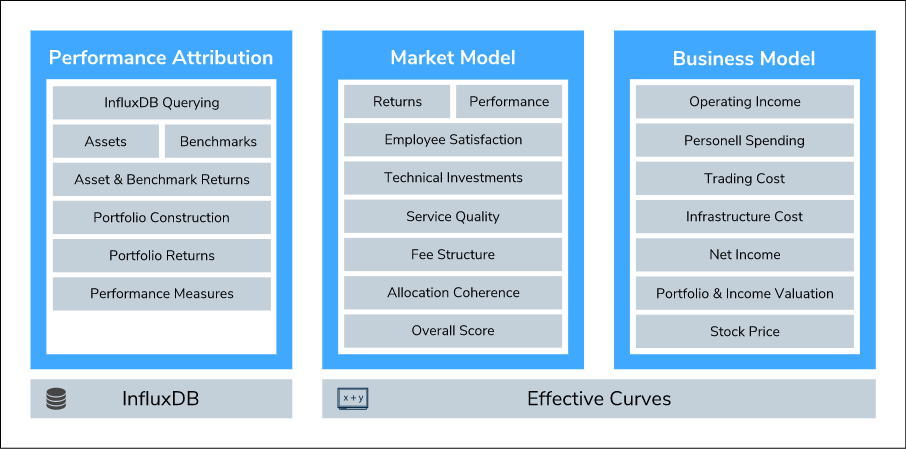
\includegraphics[width=\textwidth]{img/market_model.png}
  \caption{Market Model Overview}
  \centering
  \label{fig:market_model_overview}
\end{figure}

The PFM-Game market model is a module that produces period results based on the business decisions and portfolio allocations of teams participating in a given game. The market model is separated into several subcomponents that, when applied in sequence, produce results for a period of the game.

\subsection{Data and Data Ingestion}
The underlying data driving all portfolio-related calculations in the market model is comprised of several hunderd time-series that are stored in InfluxDB. The majority of these time-series describe asset price or return indices (i.e., asset prices normalized by the payment of dividends and other interest) as extracted from the Thomson Reuters Datastream platform. Further relevant time-series are based on macroeconomic data extracted from the FRED (Federal Reserve Economic Data) database. These data are used to calculate portfolio and benchmark returns as well as parameters of an economic forecast.

The above described data can be extracted from Datastream and FRED and ingested into an instance of InfluxDB automatically by means of a Python module that was created as an extension to the PFM-Simulation project. Data to be ingested is defined inside an assets.csv file in the following CSV format:

\begin{table}[h!]
  \begin{tabular}{lllllll}
    \toprule
    Name & Symbol  & Start Date & Market      & Data Type & Asset Type & Currency \\
    \midrule
    SWISS BOND AAA & SWBND3A & 29.12.2006 & Switzerland & RI        & BONDS      & CHF      \\
    NESTLE 'R'     & S:NESN  & 01.01.1973 & Switzerland & RI        & EQUITY     & CHF      \\
    \bottomrule
  \end{tabular}
  \centering
  \caption{Exemplary assets in a valid assets.csv definition format (optional columns omitted)}
  \label{table:assets_csv}
\end{table}

During processing of the CSV definition of all assets, the module will incrementally extend existing time-series with new data up to the current day. Time-series that were not previously available will be stored as a new series in full-length.


\subsection{Performance Attribution}
The performance attribution module is the first module in the sequence of model calculations that are applied to an incoming period scoring request (i.e., a request made by the game master on completion of a game period).

% modules/performance_attribution/influx.py
As can be seen in \ref{fig:market_model_overview}, one of the most important responsibilities of the performance attribution module is handling all data querying from the InfluxDB time-series database. Based on the incoming depot allocations of all participating teams, the module fetches all necessary asset and benchmark values from the database.\footnote{See pfm-model/api/modules/performance\_attribution/influx.py}

% modules/performance_attribution/returns.py
For all of these extracted time-series, returns need to be calculated in order to be able to continue with portfolio construction steps. All computations later in the sequence will be based on these relative return measures and not on any absolute values of the time-series.\footnote{See pfm-model/api/modules/performance\_attribution/returns.py}

% modules/performance_attribution/portfolio.py
With returns being available for all assets and their benchmarks, the performance attribution module then constructs portfolios for each team. Each team will have created one portfolio allocation for each customer type that is enabled in the current period. The module will account for this by building as many portfolios per team as there are customer types.\footnote{See pfm-model/api/modules/performance\_attribution/portfolio.py}

In addition to building portfolios for all depot allocations of the current period, the performance attribution module also computes one benchmark portfolio for each asset portfolio. These benchmark portfolios are based on the strategic asset allocation of the corresponding customer type. As the strategic asset allocation is defined once per game during period zero, the composition of these benchmark portfolios will stay the same. Only their returns will change, as the time-frame played changes with each period.

% modules/performance_attribution/returns.py
Once portfolios are built for each combination of teams and active customer types, returns need to be calculated in the same way that returns were calculated for the assets previously. However, these returns need to be additionaly weighted by the amount of money that has been invested into each asset. For example, if a team were to invest 10\% of their total assets under management in one asset and 20\% in another, the latter would influence the overall portfolio returns twice as much as the former.

% modules/performance_attribution/kpi.py
Upon completion of all previous returns calculations, the returns of assets, benchmarks, and portfolios can be combined into many useful performance measures that characterize a portfolio in different ways and allow for an easier intercomparison between teams. A byproduct of these calculations is also the new assets under management for a customer given their portfolio returns, as well as the new asset positions that a portfolio is composed of after returns are applied.For example, if one invested 50\% in one asset and 50\% in another, the new positions after returns might be 45\%-55\% if the latter asset outperforms the former.\footnote{See pfm-model/api/modules/performance\_attribution/kpi.py}

% TODO: measure list in appendix
The calculated portfolio measures include measures like the selection and tactical performance attribution that can show how much an investment into a specific asset, asset type, or market benefitted the overall portfolio. A list of all calculated measures can be found in TODO: APPENDIX. These measures could then be used by the teams to reevaluate their investments.

The final results of the performance attribution module are compiled into a suitable format and passed on to the market model module, which handles the integration of these results with business decisions as well as the grading of performance measures according to efficient curves.


\subsection{Market Model}



\subsection{Business Model}



\subsection{API Specification}
